\section{Introduction to Functions} \label{S:introfunctions}
\setcounter{previewactivity}{0}
%
\begin{previewactivity}[\textbf{Functions from Previous Courses}] \label{PA:previousfunctions} \hfill \\
One of the most important concepts in modern mathematics is that of a \textbf{function}.  In previous mathematics courses, we have often thought of a function as some sort of input-output rule that assigns exactly one output to each input.  So in this context, a \textbf{function}
\index{function}%
 can be thought of as a procedure for associating with each element of some set, called the \textbf{domain of the function},
\index{domain!of a function}%
\index{function!domain}%
 exactly one element of another set, called the \textbf{codomain of the function}.
\index{codomain}%
\index{function!codomain}%
  This procedure can be considered an input-output rule.  The function takes the input, which is an element of the domain, and produces an output, which is an element of the codomain.  In calculus and precalculus, the inputs and outputs were almost always real numbers.  So the notation $f( x ) = x^2 \sin x$ means the following:

\begin{itemize}
\item $f$  is the name of the function.

\item $f( x )$  is a real number.  It is the output of the function when the input is the real number  $x$.  For example,
\[
\begin{aligned}
  f\left( {\frac{\pi }{2}} \right) &= \left( {\frac{\pi }{2}} \right)^2 \sin \left( {\frac{\pi }
{2}} \right) \\ 
                                   &= \frac{{\pi ^2 }}{4} \cdot 1 \\ 
                                   &= \frac{{\pi ^2 }}{4}. \\ 
\end{aligned}
\]
\end{itemize}
For this function, it is understood that the domain of the function is the set  $\R$ of all real numbers.  In this situation, we think of the domain as the set of all possible inputs.  That is, the domain is the set of all possible real numbers  $x$  for which a real number output can be determined.

This is closely related to the equation  
$y = x^2 \sin x $.  With this equation, we frequently think of  $x$  as the input and  $y$  as the output.  In fact, we sometimes write  $y = f( x )$.  The key to remember is that a function must have exactly one output for each input.  When we write an equation such as  
\[
y = \dfrac{1}{2}x^3  - 1,
\]
we can use this equation to define  $y$  as a function of  $x$.  This is because when we substitute a real number for  $x$  (the input), the equation produces exactly one real number for  $y$  (the output).  We can give this function a name, such as  $g$, and write
\[
y = g( x ) = \frac{1}{2}x^3  - 1.
\]
However, as written, an equation such as  
\[
y^2  = x + 3
\]
cannot be used to define  $y$  as a function of  $x$  since there are real numbers that can be substituted for  $x$  that will produce more than one possible value of  $y$.  For example,  if  $x = 1$, then $y^2  = 4$, and  $y$  could be  $-2$  or  2.

Which of the following equations can be used to define a function with  $x \in \R$
as the input and  $y \in \R$  as the output?

\begin{multicols}{2}
\begin{enumerate}

\item $y = x^2  - 2$

\item $y^2  = x + 3$

\item $y = \dfrac{1}{2}x^3  - 1$

\item $y = \dfrac{1}{2} x\sin x$

\item $x^2  + y^2  = 4$

\item $y = 2x - 1$

\item $y = \dfrac{x}{{x - 1}}$

\end{enumerate}
\end{multicols}
\end{previewactivity}
\hbreak

\endinput

%\begin{previewactivity}[\textbf{The Definition of a Function}] \label{PA:functiondef} \hfill \\
The domain and codomain of the functions in Beginning Activity~\ref{PA:previousfunctions} is the set  $\R$ of all real numbers, or some subset of   $\R$.  In most of these cases, the way in which the function associates elements of the domain with elements of the codomain is by a rule determined by some mathematical expression.  For example, when we say that $f$  is the function such that
\[
f( x ) = \dfrac{x}{{x - 1}},
\]
then the algebraic rule that determines the output of the function  $f$  when the input is  $x$  is  
$\dfrac{x}{{x - 1}}$.  In this case, we would say that the domain of  $f$  is the set of all real numbers not equal to  1 since division by zero is not defined.

However, the concept of a function is much more general than this.  The way in which a function associates elements of the domain with elements of the codomain can have many different forms.  For example, the idea of associating with each person his or her birthday (month and day) can be thought of as a function with the domain being the set of all people and the codomain being the set of all days in a (leap) year.  So the domain and codomain can be any set and the input-output rule can be a formula, a graph, a table, a random process, a computer algorithm, or a verbal description.  We formally define the concept of a function as follows:

\begin{defbox}{function}{A \textbf{function}
\index{function}%
 from a set  $A$  to a set  $B$  is a rule that associates with every element  $x$  of the set  $A$  exactly one element of the set  $B$.  A function $f$ from  $A$  to  $B$ is also called a 
\textbf{mapping}
\index{mapping}%
 from  $A$  to  $B$.  

\newpar
When $f$ is a function from $A$ to $B$, we write $f \x A \to B$.  The set  $A$  is called the \textbf{domain}
\index{domain!of a function}%
\index{function!domain}%
of the function  $f$, and we write  $A = \text{dom}( f )$\!.\label{sym:domfunc}  The set  $B$ is called the \textbf{codomain}
\index{codomain}%
\index{function!codomain}%
of the function  $f$, and we write  $B = \text{codom}( f )$\!. \label{sym:codomain}}
\end{defbox}

\end{previewactivity}

\endinput

\begin{previewactivity}[\textbf{Some Other Types of Functions}] \label{PA:otherfunctions} \hfill \\
The domain and codomain of each of the functions in \typeu Activity~\ref*{PA:previousfunctions} are the set  $\R$ of all real numbers, or some subset of   $\R$.  In most of these cases, the way in which the function associates elements of the domain with elements of the codomain is by a rule determined by some mathematical expression.  For example, when we say that $f$  is the function such that
\[
f( x ) = \dfrac{x}{{x - 1}},
\]
then the algebraic rule that determines the output of the function  $f$  when the input is  $x$  is  
$\dfrac{x}{{x - 1}}$.  In this case, we would say that the domain of  $f$  is the set of all real numbers not equal to  1 since division by zero is not defined.

However, the concept of a function is much more general than this.  The domain and codomain of a function can be any set, and the way in which a function associates elements of the domain with elements of the codomain can have many different forms. The input-output rule for a function can be a formula, a graph, a table, a random process, or a verbal description.  We will explore two different examples in this activity.

\begin{enumerate}
  \item Let  $b$  be the function that assigns to each person his or her birthday (month and day).  The domain of the function  $b$  is the set of all people and the codomain of  $b$  is the set of all days in a leap year (i.e., January 1 through December 31, including February 29).

\begin{enumerate}
\item Explain why  $b$  really is a function.  We will call this the \textbf{birthday function}.
\index{birthday function}%

\item In 1995, Andrew Wiles
\index{Wiles, Andrew}%
 became famous for publishing a proof of Fermat's Last Theorem.  (See A. D. Aczel, \textit{Fermat's Last Theorem: Unlocking the Secret of an Ancient Mathematical Problem}, Dell Publishing, New York, 1996.)  Andrew Wiles's birthday is April 11, 1953.  Translate this fact into functional notation using the ``birthday function'' $b$.  That is, fill in the spaces for the following question marks:
\[
b( {\,?\,} ) = \,?.
\]
\item Is the following statement true or false?  Explain.

\begin{list}{}
\item For each day  $D$  of the year, there exists a person  $x$  such that  
\linebreak $b( x ) = D$.
\end{list}

\item Is the following statement true or false?  Explain.

\begin{list}{}
\item For any people  $x$  and  $y$,  if  $x$  and  $y$  are different people, then  
\linebreak $b( x ) \ne b( y )$.
\end{list}
\end{enumerate}
  
\item Let  $s$  \label{sym:sumdivisors} be the function that associates with each natural number the sum of its distinct natural number divisors.  This is called the \textbf{sum of the divisors function}.  
\index{sum of divisors function}%
For example, the natural number divisors of 6 are 1, 2, 3, and 6, and so
\[
\begin{aligned}
  s( 6 ) &= 1 + 2 + 3 + 6 \\ 
                    &= 12. \\ 
\end{aligned} 
\]
\begin{enumerate}
\item Calculate  $s( k )$ for each natural number  $k$  from  1  through 15.

%\item Are the numbers $\sqrt{5}$, $\pi$, and $-6$ in the domain of the function $s$?  What is the domain of the function  $s$?

%\item Is  $s\left( {\sqrt 5 } \right)$  defined?  Explain.  Is  $s\left( \pi  \right)$  defined?  Is  $s\left( { - 6} \right)$  defined?

\item Does there exist a natural number  $n$  such that  $s( n ) = 5$?  Justify your conclusion.

\item Is it possible to find two different natural numbers  $m$  and  $n$  such that  \linebreak
$s( m ) = s( n )$?  Explain.

\item Use your responses in (b) and (c) to determine the truth value of each of the following statements.

\begin{enumerate}
  \item For each  $m \in \mathbb{N}$, there exists a natural number  $n$  such that  
$s( n ) = m$.

  \item For all $m, n \in \mathbb{N}$, if  $m \ne n$, then  $s( m ) \ne s( n )$.
\end{enumerate}

\end{enumerate}
\end{enumerate}

\end{previewactivity}
\hbreak

\endinput


%\begin{previewactivity}[Functions from Previous Courses] \label{PA:previousfunctions} \hfill \\
A \textbf{function}
\index{function}%
 can be thought of as a procedure for associating with each element of some set, called the \textbf{domain of the function},
\index{domain!of a function}%
\index{function!domain}%
 exactly one element of another set, called the \textbf{codomain of the function}.
\index{codomain}%
\index{function!codomain}%
  This is procedure can be considered an input-output-rule.  The function takes the input, which is an element of the domain, and produces an output, which is an element of the codomain.  So the notation $f( x ) = x^2 \sin x$ means the following:

\begin{itemize}
\item $f$  is the name of the function.

\item $f( x )$  is a real number.  It is the output of the function when the input is the real number  $x$.  For example,
\[
\begin{aligned}
  f\left( {\frac{\pi }{2}} \right) &= \left( {\frac{\pi }{2}} \right)^2 \sin \left( {\frac{\pi }
{2}} \right) \\ 
                                   &= \frac{{\pi ^2 }}{4} \cdot 1 \\ 
                                   &= \frac{{\pi ^2 }}{4}. \\ 
\end{aligned}
\]
\end{itemize}
For this function, it is understood that the domain of the function is the set  $\R$ of all real numbers.  In this situation, we think of the domain as the set of all possible inputs.  That is, the domain is the set of all possible real numbers  $x$  for which a real number output can be determined.

In this situation, we often consider the function  $f$  to be a rule that assigns to each real number input  $x$  a unique output  $f( x )$.  This is closely related to the equation  
$y = x^2 \sin x $.  With this equation, we frequently think of  $x$  as the input and  $y$  as the output.  In fact, we sometimes write  $y = f( x )$.

Which of the following equations can be used to define a function with  $x \in \mathbb{R}$
as the input and  $y$  as the output?

\begin{multicols}{2}
\begin{enumerate}

\item $y = x^2  - 2$

\item $y^2  = x + 3$

\item $y = \dfrac{1}{2}x^3  - 1$

\item $y = \dfrac{1}{2} x\sin x$

\item $x^2  + y^2  = 4$

\item $y = 2x - 1$

\item $y = \dfrac{x}{{x - 1}}$

\end{enumerate}
\end{multicols}
\end{previewactivity}
\hbreak
\begin{previewactivity}[The Birthday Function] \label{PA:birthdayfunction} \hfill \\
\index{birthday function}%
The domain and codomain of the functions in Preview Activity~\ref{PA:previousfunctions} is the set  $\R$ of all real numbers, or some subset of   $\R$.  In most of these cases, the way in which the function associates elements of the domain with elements of the codomain is by a rule determined by some mathematical expression.  For example, when we say that $f$  is the function such that
\[
f( x ) = \dfrac{x}{{x - 1}},
\]
then the algebraic rule that determines the output of the function  $f$  when the input is  $x$  is  $\dfrac{x}{{x - 1}}$.  In this case, we would say that the domain of  $f$  is the set of all real numbers not equal to  1 since division by zero is not defined.

However, the concept of a function is much more general than this.  The way in which a function associates elements of the domain with elements of the codomain can have many different forms.  This input-output rule can be a formula, a graph, a table, a random process, a computer algorithm, or a verbal description.  Following is such an example.

Let  $b$  be the function that assigns to each person his or her birthday (month and day).  The domain of the function  $b$  is the set of all people and the codomain of  $b$  is the set of all days in a leap year (i.e., January 1 through December 31, including February 29).

\begin{enumerate}
\item Explain why  $b$  really is a function.

\item In 1995, Andrew Wiles
\index{Wiles, Andrew}%
 became famous for publishing a proof of Fermat's Last Theorem.  (See A. D. Aczel, \textit{Fermat's Last Theorem: Unlocking the Secret of an Ancient Mathematical Problem}, Dell Publishing, New York, 1996.)  Andrew Wiles's birthday is April 11, 1953.  Translate this fact into functional notation using the ``birthday function'' $b$.  That is, fill in the spaces for the following question marks:
\[
b( {\,?\,} ) = \,?.
\]
\item Is the following statement true or false?  Explain.

\begin{list}{}
\item For each day  $D$  of the year, there exists a person  $x$  such that  
\linebreak $b( x ) = D$.
\end{list}

\item Is the following statement true or false?  Explain.

\begin{list}{}
\item For any people  $x$  and  $y$,  if  $x$  and  $y$  are different people, then  
\linebreak $b( x ) \ne b( y )$.
\end{list}

\end{enumerate}
\end{previewactivity}
\hbreak
%
\begin{previewactivity}[The Sum of the Divisors Function] \label{PA:sumofdivisors} \hfill \\
\index{sum of divisors function}%
Let  $s$  \label{sym:sumdivisors} be the function that associates with each natural number the sum of its distinct natural number factors.  For example,
\[
\begin{aligned}
  s( 6 ) &= 1 + 2 + 3 + 6 \\ 
                    &= 12. \\ 
\end{aligned} 
\]
\begin{enumerate}
\item Calculate  $s( k )$ for each natural number  $k$  from  1  through 15.

\item Are the numbers $\sqrt{5}$, $\pi$, and $-6$ in the domain of the function $s$?  What is the domain of the function  $s$?

%\item Is  $s\left( {\sqrt 5 } \right)$  defined?  Explain.  Is  $s\left( \pi  \right)$  defined?  Is  $s\left( { - 6} \right)$  defined?

\item Does there exist a natural number  $n$  such that  $s( n ) = 5$?  Justify your conclusion.

\item Is it possible to find two different natural numbers  $m$  and  $n$  such that  \linebreak
$s( m ) = s( n )$?  Explain.

\item Are the following statements true or false?

\begin{enumerate}
  \item For each  $m \in \mathbb{N}$, there exists a natural number  $n$  such that  
$s( n ) = m$.

  \item For all $m, n \in \mathbb{N}$, if  $m \ne n$, then  $s( m ) \ne s( n )$.
\end{enumerate}

\end{enumerate}
\end{previewactivity}
\hbreak


\endinput

%
\subsection*{The Definition of a Function}
The concept of a function is much more general than the idea of a function used in calculus or precalculus.  In particular, the domain and codomain do not have to be subsets of  $\mathbb{R}$.  In addition, the way in which a function associates elements of the domain with elements of the codomain can have many different forms.  This input-output rule can be a formula, a graph, a table, a random process, a computer algorithm, or a verbal description.  Two such examples were introduced in \typeu Activity~\ref*{PA:otherfunctions}.

For the \textbf{birthday function}, 
\index{birthday function}%
 the domain would be the set of all people and the codomain would be the set of all days in a leap year.  For the \textbf{sum of the divisors function},
\index{sum of divisors function}%
 the domain is the set  $\mathbb{N}$ of natural numbers, and the codomain could also be  $\mathbb{N}$.  In both of these cases, the input-output rule was a verbal description of how to assign an element of the codomain to an element of the domain.

We formally define the concept of a function as follows:
%
\begin{defbox}{function}{A \textbf{function}
\index{function}%
 from a set  $A$  to a set  $B$  is a rule that associates with each element  $x$  of the set  $A$  exactly one element of the set  $B$.  A function from  $A$  to  $B$ is also called a 
\textbf{mapping}
\index{mapping}%
 from  $A$  to  $B$.}
\end{defbox}
%
\noindent
\textbf{Function Notation}.  When we work with a function, we usually give it a name.  The name is often a single letter, such as  $f$  or  $g$.  If  $f$  is a function from the set  $A$  to the set  $B$, we will write  $f \colon A \to B$.
\label{sym:function}%
  This is simply shorthand notation for the fact that  $f$  is a function from the set  $A$  to the set  $B$.  In this case, we also say that  $f$  maps  $A$  to  $B$.

\begin{defbox}{domainfunction}{Let  $f \colon A \to B$.  (This is read, ``Let  $f$  be a function from  $A$  to  $B$.'')  The set  $A$  is called the \textbf{domain}
\index{domain!of a function}%
\index{function!domain}%
of the function  $f$, and we write  $A = \text{dom}( f )$.\label{sym:domfunc}  The set  $B$ is called the \textbf{codomain}
\index{codomain}%
\index{function!codomain}%
of the function  $f$, and we write  $B = \text{codom}( f )$. \label{sym:codomain}
\vskip6pt
If  $a \in A$, then the element of  $B$  that is associated with  $a$  is denoted by  
$f( a )$ 
\label{sym:fofx}and is called the \textbf{image of  $\boldsymbol{a}$
\index{image!of an element}%
  under  $\boldsymbol{f}$}\!.  If  $f( a ) = b$, with  $b \in B$, then  $a$  is called a 
\textbf{preimage of  $\boldsymbol{b}$
\index{preimage!of an element}%
  for  $\boldsymbol{f}$}\!.}  
\end{defbox}
%
\noindent
\textbf{Some Function Terminology with an Example}.  When we have a function \linebreak
$f \colon A \to B$, we often write $y = f(x)$.  In this case, we consider $x$ to be an unspecified object that can be chosen from the set $A$, and we would say that  $x$  is the \textbf{independent variable}
\index{independent variable}%
\index{variable!independent}%
 of the function  $f$  and  $y$  is the \textbf{dependent variable}
\index{dependent variable}%
\index{variable!dependent}%
 of the function  $f$.

For a specific example, consider the function $g \x \mathbb{R} \to \mathbb{R}$, where  $g( x )$ is defined by the formula 
\[
g( x ) = x^2  - 2. \label{example:function}
\]
Note that this is indeed a function since given any input  $x$  in the domain, $\R$, there is exactly one output  $g( x )$ in the codomain, $\R$.  For example,
\[
\begin{aligned}
  g( { - 2} )        &= \left( { - 2} \right)^2  - 2 = 2, \\ 
  g( 5 )             &= 5^2  - 2 = 23, \\
  g( {\sqrt 2 } )    &= \left( {\sqrt 2 } \right)^2  - 2 = 0,  \\
  g( { - \sqrt 2 } ) &= \left( { - \sqrt 2 } \right)^2  - 2 = 0. \\ 
\end{aligned}
\]
So we say that the image of  $-2$ under $g$  is  2, the image of  5 under $g$ is  23, and so on.  

Notice in this case that the number  0  in the codomain has two preimages, $ - \sqrt 2 \text{ and }\sqrt 2 $.  This does not violate the mathematical definition of a function since the definition only states that each input must produce one and only one output.  That is, each element of the domain has exactly one image in the codomain.  Nowhere does the definition stipulate that two different inputs must produce different outputs.

Finding the preimages of an element in the codomain can sometimes be difficult.  In general, if  $y$ is in the codomain, to find its preimages, we need to ask, ``For which values of  $x$  in the domain will we have  
$y = g( x )$?''  For example, for the function  $g$, to find the preimages of  5, we need to find all  $x$  for which  $g( x ) = 5$.  In this case, since  $g( x ) = x^2  - 2$, we can do this by solving the equation
\[
x^2  - 2 = 5.
\]
The solutions of this equation are  $ - \sqrt 7 $  and  $\sqrt 7 $.  So for the function  $g$, the preimages of  5  are  $ - \sqrt 7 $  and  $\sqrt 7 $.  We often use set notation for this  and say that the set of preimages of 5 for the function $g$ is 
$\left\{ -\sqrt{7}, \sqrt{7} \right\}$.
%\vskip10pt

Also notice that for this function, not every element in the codomain has a preimage.  For example, there is no input  $x$  such that  $g\left( x \right) =  - 3$.  This is true since for all real numbers  $x$,  $x^2  \geq 0$  and hence  $x^2  - 2 \geq  - 2$.  This means that for all  $x$  in  $\mathbb{R}$, $g\left( x \right) \geq  - 2$.
%\noindent

Finally, note that we introduced the function $g$ with the sentence, ``Consider the function  
$g\x \mathbb{R} \to \mathbb{R}$, where  $g( x )$  is defined by the formula  
$g( x ) = x^2  - 2$.''  This is one correct way to do this, but we will frequently shorten this to, ``Let  $g\x \mathbb{R} \to \mathbb{R}$ be defined by  $g( x ) = x^2  - 2$'', or ``Let  
$g\x \mathbb{R} \to \mathbb{R}$, where  $g( x ) = x^2  - 2$.''

\begin{prog}[\textbf{Images and Preimages}] \label{pr:images} \hfill \\
Let $f\x \R \to \R$ be defined by $f(x) = x^2 - 5x$ for all $x \in \R$, and let 
$g\x \Z \to \Z$ be defined by $g(m) = m^2 - 5m$ for all $m \in \Z$.

\begin{enumerate}
\item Determine $f ( -3 )$ and $f \left( \sqrt 8 \right)$.

\item Determine $g ( 2 )$ and $g ( -2 )$.

\item Determine the set of all preimages of 6 for the function $f$\!.

\item Determine the set of all preimages of 6 for the function $g$\!.

\item Determine the set of all preimages of 2 for the function $f$\!.

\item Determine the set of all preimages of 2 for the function $g$\!.
\end{enumerate}
\end{prog}
\hbreak


\endinput

\subsection*{The Codomain and Range of a Function}
Besides the domain and codomain, there is another important set associated with a function.  The need for this was illustrated in the example of the function $g$ on page~\pageref{example:function}.  For this function, it was noticed that there are elements in the codomain that have no preimage or, equivalently, there are elements in the codomain that are not the image of any element in the domain.  The set we are talking about is the subset of the codomain consisting of all images of the elements of the domain of the function, and it is called the range of the function.
%
\begin{defbox}{rangeandimage}{Let  $f\x A \to B$.  The set  
$\left\{ {f( x ) \mid x \in A} \right\}$  is called the \textbf{range of the function}
\index{range}%
\index{function!range}%
  $\boldsymbol{f}$  and is denoted by  $\text{range}\left( f \right)$\!. \label{sym:rangef}  The range of  $f$  is sometimes called the \textbf{image of the function}  $\boldsymbol{f}$ (or the \textbf{image of} 
$\boldsymbol{A}$ \textbf{under} $\boldsymbol{f}$).}
\end{defbox}

\noindent
The range of  $f\x A \to B $ could equivalently be defined as follows:
\[
\text{range}( f ) = \left\{ { {y \in B} \mid y = f\left( x \right)\text{ for some }x \in A} \right\}\!.
\]
Notice that this means that $\text{range} (f) \subseteq \text{codom} (f)$ but does not necessarily mean that 
$\text{range} (f) = \text{codom} (f)$.  Whether we have this set equality or not depends on the function $f$.  More about this will be explored in Section~\ref{S:typesoffunctions}.
\hbreak
%
\begin{prog}[\textbf{Codomain and Range}] \label{pr:codomainandrange} \hfill 
\begin{enumerate}
\item Let  $b$  be the function that assigns to each person his or her birthday (month and day).
\begin{enumerate}
  \item What is the domain of this function?

  \item What is a codomain for this function?

  \item In \typeu Activity~\ref*{PA:otherfunctions}, we determined that the following statement is true:  For each day  $D$  of the year, there exists a person  $x$  such that  
$b( x ) = D$.
%  \begin{list}{}
%    \item For each day  $D$  of the year, there exists a person  $x$  such that  
%$b\left( x \right) = D$.
%  \end{list}
What does this tell us about the range of the function  $b$?  Explain.
\end{enumerate}

\item Let  $s$  be the function that associates with each natural number the sum of its distinct natural number factors.

\begin{enumerate}
  \item What is the domain of this function?

  \item What is a codomain for this function?

  \item In \typeu Activity~\ref*{PA:otherfunctions}, we determined that the following statement is false:

  \begin{list}{}
    \item For each  $m \in \mathbb{N}$, there exists a natural number  $n$  such that  
\linebreak $s( n ) = m$.
  \end{list}

Give an example of a natural number  $m$  that shows this statement is false, and explain what this tells us about the  range of the function  $s$\!.
\end{enumerate}

\end{enumerate}
\end{prog}
\hbreak

\endinput

\subsection*{The Graph of a Real Function}
We will finish this section with methods to visually communicate information about two specific types of functions.  The first is the familiar method of graphing functions that was a major part of some previous mathematics courses.  For example, consider the function $g \x \R \to \R$ defined by $g(x) = x^2 - 2x - 1$.

\begin{figure}[h]
\begin{center}
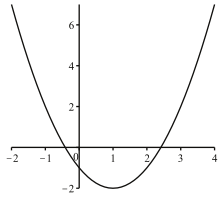
\includegraphics{figps-graphsec6-1.eps} 
\caption{Graph of $y = g( x )$, where  $g( x ) = x^2  - 2x - 1$} \label{fig:functiongraph1}
\end{center}
\end{figure}
Every point on this graph corresponds to an ordered pair  $\left( {x,\;y} \right)$ of real numbers, where  $y = g( x ) = x^2  - 2x - 1$.  Because we use the Cartesian plane when drawing this type of graph, we can only use this type of graph when both the domain and the codomain of the function are subsets of the real numbers  
$\R$.  Such a function is sometimes called a \textbf{real function}.
\label{realfunction}%
\index{real function}%
\index{function!real}%
 The graph of a real function is a visual way to communicate information about the function.  For example, the range of $g$ is the set of all  $y$-values  that correspond to points on the graph.  In this case, the graph of $g$ is a parabola and has a vertex at the point $(1, -2)$.  (\note The $x$-coordinate of the vertex can be found by using calculus and solving the equation $f ' (x) = 0$.)  Since the graph of the function $g$ is a parabola, we know that the pattern shown on the left end and the right end of the graph continues and we can conclude that the range of $g$ is the set of all $y \in \R$ such that $y \geq -2$.  That is,
\[
\text{range} (g) = \{ y \in \R \mid y \geq -2 \}.
\]
\hbreak

\begin{prog}[\textbf{Using the Graph of a Real Function}] \label{pr:graphreal} \hfill \\ 
The graph in Figure~\ref{fig:functiongraph2} shows the graph of (slightly more than) two complete periods for a function $f \x \R \to \R$, where $f(x) = A \sin (Bx)$ for some positive real number constants $A$ and $B$.
\begin{figure}[h]
\begin{center}
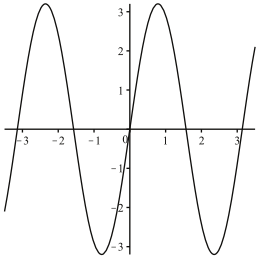
\includegraphics{figps-graph2sec6-1.eps} 
\caption{Graph of $y = f( x )$} \label{fig:functiongraph2}
\end{center}
\end{figure}
\begin{enumerate}
  \item We can use the graph to estimate the output for various inputs.  This is done by estimating the $y$-coordinate for the point on the graph with a specified $x$-coordinate.  On the graph, draw vertical lines at  $x =  - 1$  and  $x = 2$ and estimate the values of  $f( { - 1} )$  and  $f( 2 )$.
  \item Similarly, we can estimate inputs of the function that produce a specified output.  This is done by estimating the $x$-coordinates of the points on the graph that have a specified 
$y$-coordinate.  Draw a horizontal line at  $y = 2$ and estimate at least two values of  $x$  such that  
$f( x ) = 2$.
  \item Use the graph in Figure~\ref{fig:functiongraph2} to estimate the range of the function $f$.
\end{enumerate}
\end{prog}
\hbreak


\endinput


\subsection*{Arrow Diagrams}
Sometimes the domain and codomain of a function are small, finite sets.  When this is the case, we can define a function simply by specifying the outputs for each input in the domain.  For example, if we let
 $A = \left\{ {1, 2, 3} \right\}$  and let  $B = \left\{ {a, b} \right\}$, we can define a function  
$F\x A \to B$ by specifying that 
\[
F( 1 ) = a, F( 2 ) = a, \text{ and }  F( 3 ) = b.
\]
%
This is a function since each element of the domain is mapped to exactly one element in  $B$.  A convenient way to illustrate or visualize this type of function is with a so-called \textbf{arrow diagram}
\index{arrow diagram}%
 as shown in Figure~\ref{fig:arrow61-1}.
\begin{figure}[h]
\begin{center}
\scalebox{0.85}[0.85]{
\includegraphics{figps-arrow61-1x.eps}} 
\caption{Arrow Diagram for a Function} \label{fig:arrow61-1}
\end{center}
\end{figure}
An arrow diagram can be used when the domain and codomain of the function are finite (and small).  We represent the elements of each set with points and then use arrows to show how the elements of the domain are associated with elements of the codomain.  For example, the arrow from the point  2  in  $A$  to the point  $a$  in  $B$  represents the fact that  $F( 2 ) = a$.  In this case, we can use the arrow diagram in 
Figure~\ref{fig:arrow61-1} to conclude that $\text{range} (F) = \{ a, b \}$.
\hbreak

\begin{prog}[\textbf{Working with Arrow Diagrams}] \label{pr:arrow} \hfill \\
Let  $A = \left\{ {1, 2, 3, 4} \right\}$ and let  $B = \left\{ {a, b, c} \right\}$.  
\begin{enumerate}
  \item Which of the arrow diagrams in Figure~\ref{fig:arrow61-2} can be used to represent a function from  $A$  to  $B$?  Explain. \label{exer:sec61-1}
  \item For those arrow diagrams that can be used to represent a function from $A$ to $B$, determine the range of the function.
\end{enumerate}
\begin{figure}[h]
\begin{center}
\scalebox{0.85}[0.85]{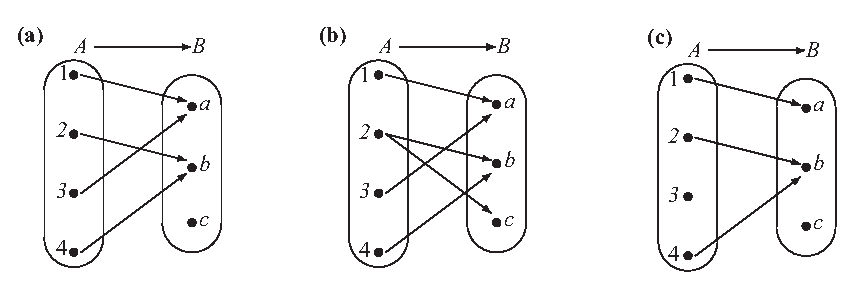
\includegraphics{figps-arrow-exer611abc.eps}} 
\caption{Arrow Diagrams} \label{fig:arrow61-2}
\end{center}
\end{figure}
\end{prog}
%\hbreak
\endinput


\endinput

\subsection*{Review of Prior Work with Functions}
One of the most important concepts in modern mathematics is that of a \textbf{function}.  In previous mathematics courses, we have often thought of a function as some sort of input-output rule that assigns exactly one output to each input.  In calculus and precalculus, the inputs and outputs were almost always real numbers.

In a more general sense, a function can be thought of as a way of associating with each element of some set, called the \textbf{domain of the function},
\index{domain!of a function}%
 exactly one element of another set, called the \textbf{codomain of the function}.
\index{codomain}%
  Using the input-output rule idea, the domain is the set of all inputs, and the codomain must contain all possible outputs.  In calculus and precalculus, the domain and codomain of a function were almost always some subset of  $\R$.  
%For these functions, the way in which a function associates elements of the domain with exactly one element of the codomain was by means of some mathematical formula.  For example, when we write something like $f\left( x \right) = x^2  + 3x$, we mean
%
%\begin{itemize}
%\item $f$  is the name of the function, and
%
%\item $f \left( x \right)$  is a real number.  It is the output of the function when the input is  $x$.
%\end{itemize}
%
%\noindent
%So $f\left( 2 \right)$ is the real number output of the function when the input is  2.  This means that
%\[
%\begin{aligned}
%  f\left( 2 \right) &= 2^2  + 3 \cdot 2 \\ 
%                    &= 10. \\ 
%\end{aligned} 
%\]
Even though the inputs and outputs are real numbers, in calculus we frequently used algebraic representations of numbers as the inputs and outputs.  For example,  $f\left( {a + h} \right)$
 represents the real number output of the function when the input is  $a + h$.  That is,
\[
\begin{aligned}
  f( {a + h} ) &= \left( {a + h} \right)^2  + 3( {a + h} ) \\ 
                          &= \left( {a^2  + 2ah + h^2 } \right) + \left( {3a + 3h} \right)\!. \\ 
\end{aligned} 
\]
The key to remember is that a function must have exactly one output for each input as we saw in Preview Activity~\ref{PA:previousfunctions}.  When we write an equation such as  
\[
y = \dfrac{1}{2}x^3  - 1,
\]
we can use this equation to define  $y$  as a function of  $x$.  This is because when we substitute a real number for  $x$  (the input), the equation produces exactly one real number for  $y$  (the output).  We can give this function a name, such as  $g$, and write
\[
y = g( x ) = \frac{1}{2}x^3  - 1.
\]
However, as written, an equation such as  
\[
y^2  = x + 3
\]
cannot be used to define  $y$  as a function of  $x$  since there are real numbers that can be substituted for  $x$  that will produce more than one possible value of  $y$.  For example,  if  $x = 1$, then  $y^2  = 4$, and  $y$  could be  $-2$  or  2.
\hbreak
%
\subsection*{Introduction to the General Concept of a Function}
The concept of a function is much more general than the idea of a function used in calculus or precalculus.  In particular, the domain and codomain do not have to be subsets of  $\mathbb{R}$.  In addition, the way in which a function associates elements of the domain with elements of the codomain can have many different forms.  This input-output rule can be a formula, a graph, a table, a random process, a computer algorithm, or a verbal description.  Two such examples were introduced in the preview activities.
%Preview Activity~\ref{PA:birthdayfunction} and Preview Activity~\ref{PA:sumofdivisors}.

For the \textbf{birthday function}
\index{birthday function}%
 in Preview Activity~\ref{PA:birthdayfunction}, the domain would be the set of all people and the codomain would be the set of all days in a leap year.  For the \textbf{sum of the divisors function}
\index{sum of divisors function}%
 in Preview Activity~\ref{PA:sumofdivisors}, the domain is the set  $\mathbb{N}$ of natural numbers, and the codomain could also be  $\mathbb{N}$.  In both of these cases, the input-output rule was a verbal description of how to assign an element of the codomain to an element of the domain.

We formally define the concept of a function as follows:
%
\begin{defbox}{function}{A \textbf{function}
\index{function}%
 from a set  $A$  to a set  $B$  is a rule that associates with every element  $x$  of the set  $A$  exactly one element of the set  $B$.  A function from  $A$  to  $B$ is also called a 
\textbf{mapping}
\index{mapping}%
 from  $A$  to  $B$.}
\end{defbox}
%
When we work with a function, we usually give it a name.  The name is often a single letter, such as  $f$  or  $g$.  If  $f$  is a function from the set  $A$  to be the set  $B$, we will write  $f\x A \to B$.
\label{sym:function}%
  This is simply shorthand notation for the fact that  $f$  is a function from the set  $A$  to the set  $B$.  In this case, we also say that  $f$  maps  $A$  to  $B$.
%
%\begin{defbox}{domainfunction}{Let  $f:A \to B$.  (This is read, ``Let  $f$  be a function from  $A$  to  $B$.'')  The set  $A$  is called the \textbf{domain}
%\index{domain}%
%\index{function!domain}%
%of the function  $f$, and we write  $A = \text{dom}\left( f \right)$  \label{sym:domfunc}.  The set  $B$ is called the \textbf{codomain}
%\index{codomain}%
%\index{function!codomain}%
%of the function  $f$, and we write  $B = \text{codom}\left( f \right)$ \label{sym:codomain}.
%\vskip6pt
%If  $x \in A$, then the element of  $B$  that is associated with  $x$  is denoted by  
%$f\left( x \right)$ 
%\label{sym:fofx}and is called the \textbf{image of  $\boldsymbol{x}$
%\index{image!of an element}%
%  under  $\boldsymbol{f}$}.  If  $f\left( x \right) = y$, with  $y \in B$, then  $x$  is called a \textbf{preimage of  $\boldsymbol{y}$
%\index{preimage!of an element}%
%  under  $\boldsymbol{f}$}.  In this case, we would also say that  $x$  is the \textbf{independent variable}
%\index{independent variable}%
%\index{variable!independent}%
% of the function  $f$  and  $y$  is the \textbf{dependent variable}
%\index{dependent variable}%
%\index{variable!dependent}%
% of the function  $f$.}
%\end{defbox}
%
\begin{defbox}{domainfunction}{Let  $f\x A \to B$.  (This is read, ``Let  $f$  be a function from  $A$  to  $B$.'')  The set  $A$  is called the \textbf{domain}
\index{domain!of a function}%
\index{function!domain}%
of the function  $f$, and we write  $A = \text{dom}( f )$\!.\label{sym:domfunc}  The set  $B$ is called the \textbf{codomain}
\index{codomain}%
\index{function!codomain}%
of the function  $f$, and we write  $B = \text{codom}( f )$\!. \label{sym:codomain}
\vskip6pt
If  $a \in A$, then the element of  $B$  that is associated with  $a$  is denoted by  
$f( a )$ 
\label{sym:fofx}and is called the \textbf{image of  $\boldsymbol{a}$
\index{image!of an element}%
  under  $\boldsymbol{f}$}\!.  If  $f( a ) = b$, with  $b \in B$, then  $a$  is called a 
\textbf{preimage of  $\boldsymbol{b}$
\index{preimage!of an element}%
  under  $\boldsymbol{f}$}\!.}  
\end{defbox}
%
When we have a function $f\x A \to B$, we often write $y = f(x)$.  In this case, we consider $x$ to be an unspecified object that can be chosen from the set $A$, and we would say that  $x$  is the \textbf{independent variable}
\index{independent variable}%
\index{variable!independent}%
 of the function  $f$  and  $y$  is the \textbf{dependent variable}
\index{dependent variable}%
\index{variable!dependent}%
 of the function  $f$.

\begin{example}[Function Terminology]\label{E:xsquaredminus2} \hfill \\
Consider the function  $g\x \mathbb{R} \to \mathbb{R}$, where  $g( x )$ is defined by the formula
\[
g( x ) = x^2  - 2.
\]
Note that this is indeed a function since given any input  $x$  in the domain, $\mathbb{R}$, there is exactly one output  $g( x )$ in the codomain, $\mathbb{R}$.  For example,
\[
\begin{aligned}
  g( { - 2} )        &= \left( { - 2} \right)^2  - 2 = 2, \\ 
  g( 5 )             &= 5^2  - 2 = 23, \\
  g( {\sqrt 2 } )    &= \left( {\sqrt 2 } \right)^2  - 2 = 0,  \\
  g( { - \sqrt 2 } ) &= \left( { - \sqrt 2 } \right)^2  - 2 = 0. \\ 
\end{aligned}
\]
So we say that the image of  $-2$  is  2, the image of  5  is  23, and so on.  

Notice in this case that the number  0  in the codomain has two preimages, $ - \sqrt 2 \text{ and }\sqrt 2 $.  This does not violate the mathematical definition of a function since the definition only states that each input must produce one and only one output.  That is, each element of the domain has exactly one image in the codomain.  Nowhere does the definition stipulate that two different inputs cannot produce the same output.

Finding the preimages of an element in the codomain can sometimes be difficult.  In general, if  $y$ is in the codomain, to find its preimages, we need to ask, ``For which values of  $x$  in the domain will we have  $y = g( x )$?''  For example, for the function  $g$, to find the preimages of  5, we need to find all  $x$  for which  $g( x ) = 5$.  In this case, since  
$g( x ) = x^2  - 2$, we can do this by solving the equation
\[
x^2  - 2 = 5.
\]
The solutions of this equation are  $ - \sqrt 7 $  and  $\sqrt 7 $.  So for the function  $g$, the preimages of  5  are  $ - \sqrt 7 $  and  $\sqrt 7 $.  We often use set notation for this  and say that the set of preimages of 5 for the function $g$ is 
$\left\{ -\sqrt{7}, \sqrt{7} \right\}$.
%\vskip10pt

Also notice that for this function, not every element in the codomain has a preimage.  For example, there is no input  $x$  such that  $g\left( x \right) =  - 3$.  This is true since for all real numbers  $x$,  $x^2  \geq 0$  and hence  $x^2  - 2 \geq  - 2$.  This means that for all  $x$  in  $\mathbb{R}$, $g\left( x \right) \geq  - 2$.
%\noindent

Finally, note that we introduced the function $g$ with the sentence, ``Consider the function  
$g\x \mathbb{R} \to \mathbb{R}$, where  $g( x )$  is defined by the formula  
$g( x ) = x^2  - 2$.''  This is one correct way to do this, but we will frequently shorten this to, ``Let  $g\x \mathbb{R} \to \mathbb{R}$ be defined by  $g( x ) = x^2  - 2$'', or ``Let  
$g\x \mathbb{R} \to \mathbb{R}$, where  $g( x ) = x^2  - 2$.''
\end{example}


\begin{prog}[Images and Preimages] \label{pr:images} \hfill \\
Let $f\x \R \to \R$ be defined by $f(x) = x^2 - 5x$ for all $x \in \R$, and let 
$g\x \Z \to \Z$ be defined by $g(m) = m^2 - 5m$ for all $m \in \Z$.

\begin{enumerate}
\item Determine $f ( -3 )$ and $f \left( \sqrt 8 \right)$.

\item Determine $g ( 2 )$ and $g ( -2 )$.

\item Determine the set of all preimages of 6 for the function $f$\!.

\item Determine the set of all preimages of 6 for the function $g$\!.

\item Determine the set of all preimages of 2 for the function $f$\!.

\item Determine the set of all preimages of 2 for the function $g$\!.
\end{enumerate}
\end{prog}
\hbreak

\subsection*{The Codomain and Range of a Function}
Besides the domain and codomain, there is another important set associated with a function.  The need for this was illustrated in Example~\ref{E:xsquaredminus2} when it was noticed that there are elements in the codomain that have no preimage or, equivalently, there are elements in the codomain that are not the image of any element in the domain.  The set we are talking about is the subset of the codomain consisting of all images of the elements of the domain of the function, and it is called the range of the function.
%
\begin{defbox}{rangeandimage}{Let  $f\x A \to B$.  The set  
$\left\{ {f( x ) \mid x \in A} \right\}$  is called the \textbf{range of the function}
\index{range}%
\index{function!range}%
  $\boldsymbol{f}$  and is denoted by  $\text{range}\left( f \right)$\!. \label{sym:rangef}  The range of  $f$  is sometimes called the \textbf{image of the function}  $\boldsymbol{f}$ (or the \textbf{image of} 
$\boldsymbol{A}$ \textbf{under} $\boldsymbol{f}$).}
\end{defbox}

\noindent
The range of  $f\x A \to B $ could equivalently be defined as follows:
\[
\text{range}( f ) = \left\{ { {y \in B} \mid y = f\left( x \right)\text{ for some }x \in A} \right\}\!.
\]
\hbreak
%
\begin{prog}[Codomain and Range] \label{pr:codomainandrange} \hfill 
\begin{enumerate}
\item Let  $b$  be the function that assigns to each person his or her birthday (month and day).
\begin{enumerate}
  \item What is the domain of this function?

  \item What is a codomain for this function?

  \item In Preview Activity~\ref{PA:birthdayfunction}, we determined that the following statement is true:  For each day  $D$  of the year, there exists a person  $x$  such that  
$b( x ) = D$.
%  \begin{list}{}
%    \item For each day  $D$  of the year, there exists a person  $x$  such that  
%$b\left( x \right) = D$.
%  \end{list}
What does this tell us about the range of the function  $b$?  Explain.
\end{enumerate}

\item Let  $s$  be the function that associates with each natural number the sum of its distinct natural number factors.

\begin{enumerate}
  \item What is the domain of this function?

  \item What is a codomain for this function?

  \item In Preview Activity~\ref{PA:sumofdivisors}, we determined that the following statement is false:

  \begin{list}{}
    \item For each  $m \in \mathbb{N}$, there exists a natural number  $n$  such that  
\linebreak $s( n ) = m$.
  \end{list}

Give an example of a natural number  $m$  that shows this statement is false, and explain what this tells us about the  range of the function  $s$\!.
\end{enumerate}

\end{enumerate}
\end{prog}
\hbreak
%

\subsection*{Arrow Diagrams}
%\begin{example} \label{E:arrowdiagram}
Let  $A = \left\{ {1, 2, 3} \right\}$  and let  $B = \left\{ {a, b} \right\}$.  Define the function  $F\x A \to B$ by  
\[
F( 1 ) = a, F( 2 ) = a, \text{ and }  F( 3 ) = b.
\]
%
This is a function since each element of the domain is mapped to exactly one element in  $B$.  This function is defined by simply specifying the outputs for each input in the domain.  
A convenient way to illustrate or visualize this type of function is with an \textbf{arrow diagram}
\index{arrow diagram}%
 as shown in Figure~\ref{fig:arrow61-1}.
\begin{figure}[h]
\begin{center}
\scalebox{0.85}[0.85]{
\includegraphics{figps-arrow61-1x.eps}} 
\caption{Arrow Diagram for a Function} \label{fig:arrow61-1}
\end{center}
\end{figure}

An arrow diagram can be used when the domain and codomain of the function are finite (and small).  We represent the elements of each set with points and then use arrows to show how the elements of the domain are associated with elements of the codomain.  For example, the arrow from the point  2  in  $A$  to the point  $a$  in  $B$  represents the fact that  $F( 2 ) = a$.
%\end{example}
%\hbreak

\begin{prog}[Working with Arrow Diagrams] \label{pr:arrow} \hfill \\
Let  $A = \left\{ {1, 2, 3, 4} \right\}$ and let  $B = \left\{ {a, b, c} \right\}$.  Which of the following arrow diagrams can be used to represent a function from  $A$  to  $B$?  Explain. \label{exer:sec61-1}

\begin{figure}[h]
\begin{center}
\scalebox{0.85}[0.85]{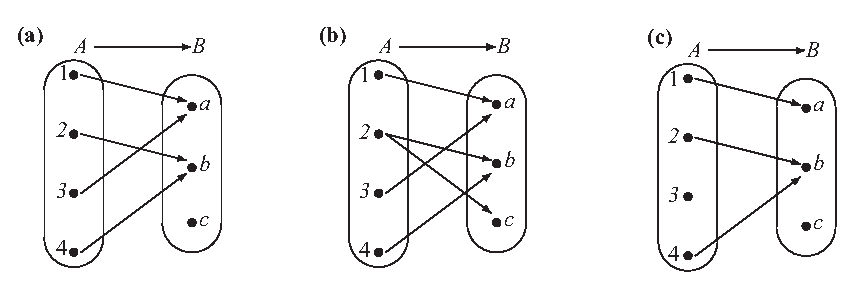
\includegraphics{figps-arrow-exer611abc.eps}} 
%\caption{Arrow Diagram for a Function} \label{fig:arrow61-1}
\end{center}
\end{figure}

%\begin{figure}[h]
%\begin{center}
%\scalebox{0.85}[0.85]{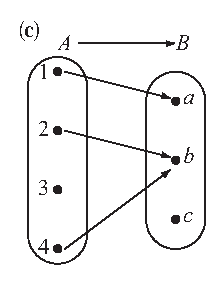
\includegraphics{figps-arrow-exer611c.eps}} 
%%\caption{Arrow Diagram for a Function} \label{fig:arrow61-1}
%\end{center}
%\end{figure}
\end{prog}
%\hbreak

%
%\enlargethispage{-\baselineskip}

%
%\begin{example} \label{E:functiontwo}
\subsection*{A Function of Two Variables} \label{ss:functiontwovar}
In Section~\ref{S:cartesian}, we learned how to form the Cartesian product of two sets.  Since a Cartesian product is a set, it could be used as the domain or codomain of a function.  For example, we could use  $\mathbb{Z} \times \mathbb{Z}$ as the domain of a function as follows:
%
\begin{center}
Let $f\x \mathbb{Z} \times \mathbb{Z} \to \mathbb{Z}$ be defined by  
$f( {m, n} ) = 2m + n$.
\end{center}

\begin{itemize}
\item Technically, an element of  $\mathbb{Z} \times \mathbb{Z}$  is an ordered pair, and so we should write  $f( {( {m, n} )} )$ for the output of the function  $f$   when the input is  
$\left( {m, n} \right)$.  However, the double parentheses seem unnecessary in this context and there should be no confusion if we write  $f( {m, n} )$ for the output of the function  $f$   when the input is  $\left( {m, n} \right)$.  So, for example, we simply write

\[
\begin{aligned}
  f( {3, 2} )    &= 2 \cdot 3 + 2 = 8,\text{ and} \\ 
  f( { - 4, 5} ) &= 2 \cdot \left( { - 4} \right) + 5 =  - 3. \\ 
\end{aligned} 
\]
\item Since the domain of this function is $\Z \times \Z$ and each element of $\Z \times \Z$ is an ordered pair of integers, we frequently call this type of function a \textbf{function of two variables}.
\index{function!of two variables}%
\end{itemize}

Finding the preimages of an element of the codomain, $\mathbb{Z}$, involves solving an equation with two variables.  For example, to find the preimages of  $0 \in \mathbb{Z}$, we need to find all ordered pairs  $\left( {m, n} \right) \in \mathbb{Z} \times \mathbb{Z}$ such that 
$f( {m, n} ) = 0$.  This means that
\[
2m + n = 0.
\]
Three such ordered pairs are  $\left( {0, 0} \right)$, $\left( {1,  - 2} \right)$, and  $\left( { - 1, 2} \right)$.  In fact, whenever we choose an integer value for  $m$ , we can find a corresponding integer  $n$  such that  $2m + n = 0$.  This means that  0  has infinitely many preimages.  One way to communicate this is to use set builder notation and say that the following set consists of all of the preimages of  0:
\[
\left\{ { {\left( {m, n} \right) \in \mathbb{Z} \times \mathbb{Z} } \mid 2m + n = 0} \right\} = \left\{ { {\left( {m, n} \right) \in \mathbb{Z} \times \mathbb{Z} } \mid n =  - 2m} \right\}\!.
\]
The second formulation for this set was obtained by solving the equation  
\linebreak $2m + n = 0$
for  $n$.
%\end{example}

\begin{prog}[Working with a Function of Two Variables] \label{pr:function-two} \hfill \\
Let $g\x \mathbb{Z} \times \mathbb{Z} \to \mathbb{Z}$ be defined by  
$g( {m, n} ) = m^2 - n$ for all $\left(m, n \right) \in \Z \times \Z$.

\begin{enumerate}
\item Determine $g(0, 3)$, $g(3,-2)$, $g(-3, -2)$, and $g(7, -1)$.
\item Determine the set of all preimages of the integer 0 for the function $g$.  Write your answer using set builder notation.
\item Determine the set of all preimages of the integer 5 for the function $g$.  Write your answer using set builder notation.
\end{enumerate}

\end{prog}
\hbreak

\begin{activity}[Creating Functions with Finite Domains] \label{A:creatingfunctions} \hfill

Let  $A = \left\{ {a,b,c,d} \right\}$, $B = \left\{ {a,b,c} \right\}$, and  
$C = \left\{ {s,t,u,v} \right\}$.  In each of the following exercises, draw an arrow diagram to represent your function when it is appropriate.
\begin{enumerate}
\item Create a function  $f\x A \to C$ whose range is the set   $C$  or explain why it is not possible to construct such a function.

\item Create a function  $f\x A \to C$ whose range is the set  $\left\{ {u, v} \right\}$ or explain why it is not possible to construct such a function.

\item Create a function  $f\x B \to C$ whose range is the set   $C$  or explain why it is not possible to construct such a function.

\item Create a function  $f\x A \to C$ whose range is the set  $\left\{ u \right\}$ or explain why it is not possible to construct such a function.

\item If possible, create a function  $f\x A \to C$  that satisfies the following condition:
\begin{list}{}
\item For all  $x, y \in A$,  if  $x \ne y$, then  $f( x ) \ne f( y )$.
\end{list}
If it is not possible to create such a function, explain why.

\item If possible, create a function  $f\x A \to \left\{ {s, t, u} \right\}$ that satisfies the following condition:

\begin{list}{}
\item For all  $x, y \in A$,  if  $x \ne y$, then  $f( x ) \ne f( y )$.
\end{list}

If it is not possible to create such a function, explain why.
\end{enumerate}
\end{activity}
\hbreak
%\subsection*{The Graph of a Real Function}
\begin{activity}[The Graph of a Real Function] \label{A:usingagraph} \hfill \\
The function  $g\x \mathbb{R} \to \mathbb{R}$, where  $g( x )$ is defined by  
$g\left( x \right) = x^2  - 2$, can be represented by a graph.  We have graphed such functions in previous mathematics courses, and the familiar graph of this function is shown in Figure~\ref{fig:functiongraph1}.

\begin{figure}[h]
\begin{center}
\includegraphics{figps-graph1.eps} 
\caption{Graph of $y = g( x )$, where  $g( x ) = x^2  - 2$} \label{fig:functiongraph1}
\end{center}
\end{figure}

Every point on this graph corresponds to an ordered pair  $\left( {x,\;y} \right)$ of real numbers, where  $y = g( x ) = x^2  - 2$.  Because we use the Cartesian plane when drawing this type of graph, we can only use this type of graph when both the domain and the codomain of the function are subsets of the real numbers  $\mathbb{R}$.  Such a function is sometimes called a \textbf{real function}.
\index{real function}%
\index{function!real}%
 The graph of a real function is a visual way to communicate information about the function.  
The graph of a real function  \linebreak
$f\x \mathbb{R} \to \mathbb{R}$ is shown in Figure~\ref{fig:functiongraph2}.
%\begin{figure}[h]
%\begin{center}
%\includegraphics[6.6cm,4.8cm]{figgraph2.bmp}
%\caption{Graph of $y = f\left( x \right)$.} \label{fig:functiongraph2}
%\end{center}
%\end{figure}
\begin{figure}[h]
\begin{center}
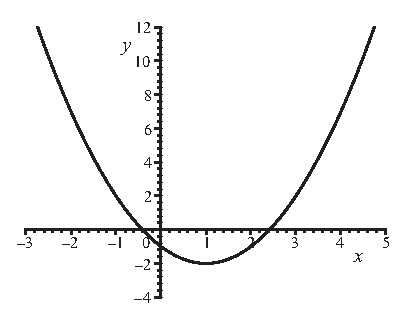
\includegraphics{figps-yfunctionx.eps}
\caption{Graph of $y = f\left( x \right)$} \label{fig:functiongraph2}
\end{center}
\end{figure}
\begin{enumerate}
\item We can use the graph to estimate the output for various inputs.  This is done by estimating the $y$-coordinate for the point on the graph with a specified $x$-coordinate.  On the graph, draw vertical lines at  $x =  - 1$  and  $x = 2$ and estimate the values of  
$f( { - 1} )$  and  $f( 2 )$.

\item Similarly, we can estimate the inputs of the function that produce a specified output.  This is done by estimating the $x$-coordinates of the points on the graph that have a specified 
$y$-coordinate.  Draw a horizontal line at  $y = 4$ and estimate the value(s) of  $x$  such that  $f( x ) = 4$.

\item If certain conditions are satisfied, the graph also gives us an indication of the range of the function.  The range is the set of all  $y$-values  that correspond to points on the graph.  By stating that  $f$  is a function with domain and codomain equal to  $\mathbb{R}$, $f\x \mathbb{R} \to \mathbb{R}$, we can assume that the graph shown is only a portion of the entire graph of the function.  If we assume that the graph of the function continues the pattern shown on the left end and the right end, what is the range of this function?  Note that we can only estimate the range since  we will have to estimate the $y$-coordinate of the low point on the graph.

\item The graph shown could also be considered to be the entire graph for the function  
$k\x \left[ { - 3, 5} \right] \to \mathbb{R}$.  In this case, what is the range of the function  $k$?
\end{enumerate}

\end{activity}
\hbreak

\endinput











\begin{center}
\setlength{\unitlength}{0.3cm}
\begin{picture}(14,14)
\put(2,6){\oval(4,12)}
\put(10,6){\oval(4,8)}

\put(2,2){\circle*{.5}}
\put(2,6){\circle*{.5}}
\put(2,10){\circle*{.5}}

\put(10,4){\circle*{.5}}
\put(10,8){\circle*{.5}}

\put(1,1.8){3}
\put(1,5.8){2}
\put(1,9.8){1}
\put(10.5,3.8){$b$}
\put(10.5,7.8){$a$}

\put(1.8,12.5){$A$}
\put(10,12.5){$B$}

\put(3,12.8){\vector(1,0){7}}
\put(6,13.2){$F$}

\put(2.5,2){\vector(4,1){7.1}}
\put(2.5,6){\vector(4,1){7.1}}
\put(2.5,10){\vector(4,-1){7.1}}

\end{picture}
\end{center}

\endinput

